% Template informe grupal CAMBIAR INFORMACION EN PORTADA GRUPO Y CONFIG DADO EL DEPARTAMENTO
\documentclass[11pt,letterpaper,spanish,notitlepage]{report}
\usepackage{physics}

\usepackage[utf8x]{inputenc} % Windows
\usepackage[spanish]{babel} % Windows

%\usepackage{ucs} % Para ubuntu
%\usepackage[utf8x]{inputenc} % Para ubuntu
%\usepackage[activeacute,spanish]{babel} % Para ubuntu

\usepackage{anysize}
\marginsize{4.25cm}{2cm}{2cm}{2cm}
\usepackage{amsmath}
\usepackage{amsfonts}
\usepackage{amssymb}
\usepackage{fancyhdr}
\usepackage{flowfram}
\usepackage{float}
\usepackage{multirow}
\usepackage{multicol}
\usepackage{setspace}
\usepackage{wrapfig}
\usepackage{longtable}
\usepackage{tabularx}
\usepackage{booktabs}
\usepackage[table]{xcolor}
\usepackage{titlesec}
\usepackage{alltt}
\usepackage{tocbibind}
%\usepackage{caption}
%\usepackage{subcaption}
\usepackage{subfig}
\usepackage{subfloat}

%\usepackage[activeacute,spanish,es-tabla]{babel}
\usepackage{graphicx}

% Top margin above chapter
\usepackage{titlesec}
\titlespacing*{\chapter}{0pt}{-70pt}{20pt}
\titleformat{\chapter}[display]{\normalfont\huge\bfseries}{\chaptertitlename\ \thechapter}{20pt}{\Huge}



%%%%%%%%%%%%%%%%%%%%%%%%%%%%%%%%%%%%%%%
%codigo de color
\usepackage{color}
\definecolor{gray51}{rgb}{0.51,0.51,0.51}
\definecolor{gray71}{rgb}{0.71,0.71,0.71}
\newcommand{\HRule}{\rule{\linewidth}{.4mm}}

\usepackage{listings}
\lstset{
	tabsize=4,
	language=Octave,
        basicstyle=\scriptsize,
        %upquote=true,
        aboveskip={1.5\baselineskip},
        columns=fixed,
	numbers=left,
        showstringspaces=false,
        extendedchars=true,
        breaklines=true,
        prebreak = \raisebox{0ex}[0ex][0ex]{\ensuremath{\hookleftarrow}},
	frame=false,
        showtabs=false,
        showspaces=false,
        showstringspaces=false,
        identifierstyle=\ttfamily,
        keywordstyle=\color[rgb]{0,0,1},
        commentstyle=\color[rgb]{0.133,0.545,0.133},
        stringstyle=\color[rgb]{0.627,0.126,0.941},
%	language=matlab
}

%%%%%%%%%%%%%%%%%%%%%%%%%%%%%%%%%%%%%%%
% para insertar codigo usar:
%\lstinputlisting[title=\textbf{Código Fuente: archivo}]{codigo.m}
%%%%%%%%%%%%%%%%%%%%%%%%%%%%%%%%%%%%%%%

\addtolength{\voffset}{-2.5 cm}
\addtolength{\hoffset}{-2 cm}
\setlength{\marginparwidth}{0 cm}
\addtolength{\headsep}{+1.5cm}
\setlength{\evensidemargin}{0cm}

%ancho texto
\setlength{\textwidth}{6.7 in}

%largo texto
\setlength{\textheight}{8.7 in}

\setlength{\headheight}{48pt}

\usepackage[pdfborder={0 0 0}]{hyperref}
\pagestyle{fancy}
\fancyhead[l]{\footnotesize Universidad de Chile - Facultad de Ciencias Físicas y Matemáticas\\
EL4003- Señales y Sistemas II\\
Prof. Manuel Duarte, Prof. Jorge Silva\\Prof. Aux. Alejandro Veragua\\  Semestre Otoño 2017}
\fancyhead[r]{
\includegraphics[scale=0.33]{fcfm.png}}
\fancyfoot[r]{\thepage}
\fancyfoot[c]{}

%\newcommand{\portadagrupo}[9]{
\begin{titlepage}

% Upper part of the page
 

{
\begin{wrapfigure}{l}{.8cm}
\vspace{-.7cm}

\includegraphics[width=4.7cm]{fcfm}
\end{wrapfigure}

\textsc{\color{red}\hspace{3cm}Departamento de Ingeniería Eléctrica}\\
\textsc{\color{gray51}\hspace{3.6cm}Facultad de Ciencias Físicas y Matemáticas}\\
\textsc{\color{gray51}\hspace{3.6cm}Universidad de Chile}\\
\textsc{\color{gray51}\hspace{3.6cm}\small El3001 - Análisis y Diseño de Circuitos Eléctricos}\\
}
% T�tulo
\begin{center}
~\\[4.5cm]
{\color{gray71}\textsc{#3}}
\HRule~ \\[0.4cm]
{ \Huge \textup \bfseries  #1}\\[0.4cm]
{ \Large \textup{#2}}\\[0.2cm]
\HRule ~\\[2cm]
\end{center}
\begin{minipage}{.5\textwidth}
~
\end{minipage}
\begin{minipage}{.5\textwidth}
\begin{flushright}
\begin{tabular}{l}
\emph{Profesor:} \\
{\small Pablo Estévez}\\[0.3cm]
\emph{Auxiliar:} \\
{\small Joaquín Díaz Peña}\\[0.3cm]
\emph{Ayudantes:} \\
{\small #4}\\
{\small #5}\\
{\small #6}\\[0.3cm]
\emph{Integrantes:}\\
{\small #7}\\
{\small #8}\\
{\small #9}\\[.3cm]
\emph{Fecha:}\\
{\small \today}
\end{tabular}
\end{flushright}
\end{minipage}
\end{titlepage}
}


\begin{document}
%\renewcommand{\tablename}{Tabla}
%\renewcommand{\figurename}{Figura}
%\renewcommand{\thetable}{\arabic{section}.\arabic{table}}
%\renewcommand{\thefigure}{\arabic{section}.\arabic{figure}}
%\renewcommand{\listtablename}{Índice de Tablas}
%\renewcommand{\listfigurename}{Índice de Figuras}

\begin{center}
    \title\huge\textbf{Ejercicio 1\\Informe Técnico\\ “Sistema de Estanque de Retroalimentación"\\
Francisca P. Herrera Rojas\\
18.263.316.-k}\\
    \vspace{8mm}
\end{center}

\begin{figure}[h!]
    \centering
    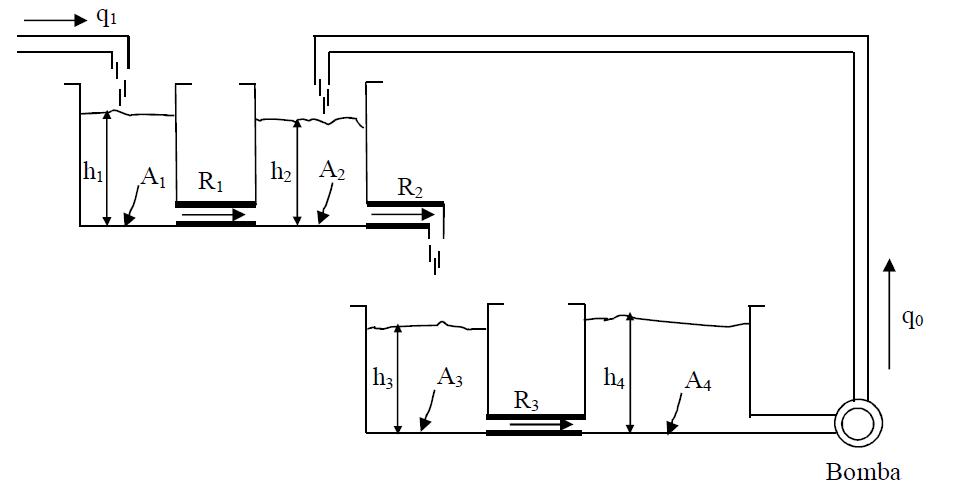
\includegraphics[scale=0.7]{Ejercicio1.png}%COLOCAR NUEVA FOTO
    \caption{Interconexión de estanques con retroalimentación }
    \label{fig:my_label}
\end{figure}

\textbf{Introducción}\\
\justify Se considera el sistema hidráulico, consistente de 4 estanques interconectados por los cuales circula un fluido. $R_{1}$, $R_{2}$, $R_{3}$ representan las restricciones al paso del fluido por los ductos modeladas como proporcionales a la raíz de la diferencia de presiones a ambos lados de la restricción. Una bomba eléctrica de velocidad variable impulsa el fluido desde el estanque 4 hacia el estanque 2 que se encuentra en la parte superior.\\

\textbf{Desarrollo}\\

\justify Utilizando el principio de conservación y una serie de hipótesis simplificatorias, se puede definir una serie de ecuaciones y diversas variables del sistema con las cuales se creara un modelo matemático que para luego lograr obtener un sistema linealizado que posteriormente permitira analizar la evolucion temporal del sistema.\\

\newpage

\textbf{Hipótesis Simplificatorias}\\
\justify A continuación, se enuncian las principales hipótesis simplificatorias utilizadas para el modelamiento del sistema:\\
\begin{itemize}
    \item El sistema se encuentra aislado, por lo que no existen fugas del fluido entre las paredes de los estanques.
    \item No existe evaporación del fluido en el medio.
     \item La densidad, $\rho$, es constante en todo el fluido ya que se trata de un fluido incompresible.
     \item No existe roce entre el fluido y las paredes de los estanques.
     \item Se supone que el sistema se encuentra en la tierra, por tanto la gravedad $g$= 9,8 $\frac{m}{s^2}$.
     \item Se conserva la energía del sistema y el volumen del fluido no sufre variaciones.
     \item Los caudales son constantes.
     \item Las secciones de los 4 estanques son iguales a 6$m^{2}$.
     \item El fluido en los estanque corresponde a agua que tiene un $rho$ igual a 1000$\frac{kg}{m^{3}}$.
\end{itemize}

\textbf{Principio de Bernoulli}\\
\justify Este principio enunciado por primera vez por Daniel Bernoulli en su obra $Hidrodinamica$, publicada en el año 1738, establece que un liquido incompresible y carente de viscosidad, la suma de la presión hidrostática, la energía cinética por unidad de volumen y la energía potencia gravitatoria por unidad de volumen, es constante a lo largo de todo el circuito. 



\begin{equation}\label{eq:venturi}
    P_{1}+\rho gh_{1}+\frac{1}{2}\rho {v_{1}}^2 = P_{2}+\rho gh_{2}+\frac{1}{2}\rho {v_{2}}^2
\end{equation}




\justify \textbf{$P$} corresponde a la presión hidrostática, \textbf{$\rho$} la densidad, \textbf{$g$} la aceleración de la gravedad, \textbf{$h$} la altura del punto y \textbf{$v$} la velocidad del fluido en ese punto. Los subíndices corresponde a 2 puntos del circuito, por tanto dicha expresión toma el mismo valor en cualquier par de puntos a lo largo del circuito.\\

\textbf{Efecto Venturi}\\
\justify El efecto Venturi fue descubierto por el físico italiano Giovanni Battista Venturi, este efecto se explica a partir del Principio de Bernoulli y el principio de continuidad de masa. Este establece que si el caudal del fluido es constante pero la sección por la que este se desplaza disminuye, entonces la velocidad por la que atraviesa esta sección aumenta. Luego por el teorema de la conservación de la energía mecánica si la energía cinética aumenta, la energía establecida por la presión disminuye.

\begin{equation}
    \frac{{V_{1}}^2}{2g}+\frac{P_{1}}{\rho g}+z_{1} = \frac{{V_{2}}^2}{2g}+\frac{P_{2}}{\rho g}+z_{2}
\end{equation}

\justify \textbf{$V$} corresponde a la velocidad del flujo en la sección del circuito considerada, al igual que \textbf{$P$} para la presión. \textbf{$g$} corresponde a la constante de aceleración gravitatoria, \textbf{$\rho g$} es el peso especifico del liquido (como el fluido que esta en estudio es incompresible, este valor se mantiene constante),y finalmente \textbf{$z$} corresponde a la altura.

\newpage 


\textbf{Modelado del Sistema}

\justify Las variables $R_{1}$, $R_{2}$, $R_{3}$, $R_{4}$ representan restricciones a las que esta sometido el paso del fluido por los ductos entre los estanque, estas restricciones son proporcionales a la raíz de la diferencia entre las diferencias de presión entre ambos lados de la restrcción. Esta relación corresponde a la del caudal del un fluido, por lo que se dejara expresado de la siguiente manera:\\
\begin{align*}
    Q &= R_{x}\sqrt{P_{y}-P_{z}}\\
    Q &= R_{x}\sqrt{\rho gh_{y}-\rho gh_{z}}\\
    Q &= R_{x}\sqrt{\rho g}\sqrt{h_{y}-h_{z}}\\
     Q &= k_{x}\sqrt{h_{y}-h_{z}}
\end{align*}
    


\justify Estanque 1:\\
\begin{equation}
    Q_{12}=k_{1}\sqrt{h_{1}-h_{2}}
\end{equation}
\begin{equation}
    A_{1}\frac{dh_{1}}{dt} = q_{1}-R_{1}Q_{12}
\end{equation}

\justify Estanque 2:
\begin{equation}
    Q_{23}=k_{1}\sqrt{h_{2}}
\end{equation}
\begin{equation}
    A_{2}\frac{dh_{2}}{dt} = (R_{1}Q_{12}+q_{0})-R_{2}Q_{23}
\end{equation}

\justify Estanque 3:
\begin{equation}
    Q_{34}=k_{3}\sqrt{h_{3}-h_{4}}
\end{equation}
\begin{equation}
    A_{3}\frac{dh_{3}}{dt} = R_{2}Q_{23}-R_{3}Q_{34}
\end{equation}

\justify Estanque 4:
\begin{equation}
    Q_{x}= \sqrt{\rho gh_{4}}
\end{equation}

\begin{equation}
    A_{4}\frac{dh_{4}}{dt} = R_{3}Q_{x}-q_{0}
\end{equation}




\justify La modelación de la bomba de velocidad variable se realiza utilizando la ecuación del efecto Venturi~\ref{eq:venturi} y considerando las siguientes variables:
\begin{itemize}
    \item $z_{1}$ como la altura a la que se encuentra el fluido en el estanque 4, $h_{4}$\\
    \item $x$ corresponde a la altura a la que se encuentra la salida del ducto de retroalimentación respecto al estanque 4.
    \item $V_{b}$ corresponde a la velocidad variable de la bomba.
    \end{itemize}

\begin{equation}
    q_{0} = \sqrt{\frac{4\rho gh_{4}+V_{b}^{2}\rho-2\rho gx}{2}}
\end{equation}


\newpage


   
\textbf{Variables del Sistema}
 \justify Se separan en 2 grandes grupos:\\ %COMPLETAR
 \textbf{Variables internas}:
    \begin{itemize}
     \item Variables de entrada: $q_{1}$
     \item Variables de salida: $q_{0}$
     \end{itemize}
 \textbf{Variables externas}:
 \begin{itemize}
     \item Variables de estado: $h_{1}$, $h_{2}$, $h_{3}$, $h_{4}$
     \item Parámetros:$A_{1}$, $A_{2}$, $A_{3}$, $A_{4}$, $\rho$, $g$,$k_{1}$, $k_{2}$, $k_{3}$, $V_{b}$
     \end{itemize} 
 \justify Las variables de estado corresponden a las variables que describen la evolución del sistemas y que relacionan las variables de salida con las de entrada.\\

 
    \begin{table}[h!]
    \centering
    \begin{tabular}{|c|c|}
       \hline
       Variable  & mks \\
         \hline
        $V_{b}$ & $\frac{m}{s}$\\ \hline
        $q_{1}$,$q_{0}$ & $\frac{m^{3}}{s}$ \\ \hline
        $A_{1}$,$A_{2}$,$A_{3}$,$A_{4}$ & $m^2$ \\ \hline 
        $g$&$\frac{kgm}{s^{2}}$\\ \hline
        $h_{1}$, $h_{2}$,$h_{3}$,$h_{4}$,x & m  \\\hline
        $\rho$ & $\frac{kg}{m^{3}}$\\ \hline
         $R_{1}$,$R_{2}$,$R_{3}$ & -\\ \hline 
        
    
    \end{tabular}
    \caption{Variables con sus respectivas unidades MKS}
    \label{tab:my_label}
\end{table}
  

 \textbf{Características del Sistema}\\
    \justify Los sistemas, en general, se pueden clasificar en función de diversos criterios, como la naturaleza de los parámetros, variables, etc. Para el sistema de la Fig.1 se tienen las siguientes características.\\
    \begin{itemize}
    
    \item \textbf{Sistema Artificial}: Los estanques, la bomba eléctrica y las partes que constituyen el sistema, son imposibles de encontrar en la naturaleza como tal.
    
    \item \textbf{Sistema Deterministico}: El sistema consta de variables cuya cuantificación es exacta y están determinadas para todo instante de tiempo. 
    
    \item \textbf{Sistema Monovariable}: El sistema cuenta con una entra ($q_{1}$) y una única variable de salida $q_{0}$.
    
    \item \textbf{Sistema de Variable Continua}:Las variables pueden tomar todos los valores dentro de un conjunto de valores posibles.
    
    \item \textbf{Sistema de Tiempo Continuo}: Entre sus ecuaciones de modelado tiene ecuaciones diferenciales.
    
     \item \textbf{Sistema Variable Concentrada}: Los atributos no dependen de coordenadas espaciales.
     
     \item \textbf{Sistema Variable en el Tiempo}: Para ser considerada invariante en el tiempo, los parámetros no dependen del tiempo.
    
    \item \textbf{Sistema Causal}: es causal si la salida en t depende una entrada para t'$<$t (salida correspondiente a estanque 4).
    
    \item\textbf{Sistema no lineal}:
    
    \item \textbf{Sistema con Memoria}: El sistema en el instante t depende de las entrada aplicada en -$\infty$ y t.
     \end{itemize}



\textbf{Linealización del sistema}\\
\justify Ahora se procede a linealizar el sistema, para esto se realiza un desarollo de Taylor y la obtención de los puntos de operación (equilibrio).\\
\begin{align*}
    \dot x &= Ax+Bu\\
 \end{align*}




\justify Los puntos de equilibrio son los siguiente $\dot h_{1}$ $=$ $\dot h_{2}$ $=$ $\dot h_{3}$ $=$ $\dot h_{4}$ $=$ 0, estos valores se reemplazan en las ecuaciones modeladas anteriormente.\\


\begin{align*}
\dot h_{1} &= \frac{q_{1}}{A_{1}} -\frac{Q_{12}}{A_{1}}\\
\dot h_{2} &= \frac{Q_{12}-q_{0}}{A_{2}} - \frac{Q_{23}}{A_{2}}\\
\dot h_{3} &= \frac{Q_{23}}{A_{3}}- \frac{Q_{34}}{A_{3}}\\
\dot h_{4} &= \frac{Q_{x}-q_{0}}{A_{4}}
\end{align*}

\justify Se reemplazan los valores de los caudales $Q_{12}$, $Q_{23}$, $Q_{34}$, $Q_{x}$, $q_{0}$ por las ecuaciones (3), (5),(7),(9)y(11), respectivamente:\\


\begin{align*}
\dot h_{1} &= \frac{q_{1}}{A_{1}} -\frac{k_{1}\sqrt{h_{1}-h_{2}}}{A_{1}}\\
\dot h_{2} &= \frac{k_{1}\sqrt{h_{1}-h_{2}}-q_{0}}{A_{2}} - \frac{k_{1}\sqrt{h_{2}}}{A_{2}}\\
\dot h_{3} &= \frac{k_{1}\sqrt{h_{2}}}{A_{3}}- \frac{k_{3}\sqrt{h_{3}}-h_{4}}{A_{3}}\\
\dot h_{4} &= \frac{\sqrt{\rho gh_{4}}}{A_{4}}-\frac{1}{A_{4}}\sqrt{\frac{V_{b}^{2}\rho +4\rho gh_{4}-2\rho gx}{2}}
\end{align*}


\newpage



\justify Despejando se obtienen los valores correspondientes a los puntos de operación del sistema:\\
\begin{equation}
    \bar h_{1} &= \frac{q_{1}^{2}}{k_{1}^{2}}+\frac{1}{k_{1}^{2}}(q_{1}+\sqrt{g\rho x-\frac{V_{b}^{2}\rho}{2}})^{2}
\end{equation}

\begin{equation}
    \bar h_{2} &= \frac{1}{k_{1}^{2}}(q_{1}+\sqrt{g\rho x-\frac{V_{b}^{2}\rho}{2}})^{2}
\end{equation}

\begin{equation}
    \bar h_{3} &=  \frac{1}{k_{3}^{2}}(q_{1}+\sqrt{g\rho x-\frac{V_{b}^{2}\rho}{2}})+ \frac{2gx-V_{b}^{2}}{2g}
\end{equation}

\begin{equation}
    \bar h_{4} &= \frac{2gx-V_{b}^{2}}{2g}
\end{equation}


\justify Las ecuaciones $\dot h_{x}$ obtenidas en la parte superior serán denominadas $f_{x}$ y seran utilizadas para calcular la matriz A que tiene forma de un Jacobiano:\\



\begin{equation}
    A=\begin{bmatrix}
 \frac{\partial f_{1}}{\partial x_{1}}& \cdots  & \frac{\partial f_{1}}{\partial x_{n}}\\ 
\vdots  & \ddots  &\vdots  \\ 
\frac{\partial f_{n} }{\partial x_{1}} & \cdots  & \frac{\partial f_{n} }{\partial x_{n}}
\end{bmatrix}
\end{equation}



\begin{equation}
    A=\begin{bmatrix}
\frac{-k_{1}}{2A_{1}\sqrt{h_{1}-h_{2}}}&\frac{k_{1}}{2A_{1}\sqrt{h_{1}-h_{2}}} &0 &0 \\ 
\frac{k_{1}}{2A_{2}\sqrt{h_{1}-h_{2}}}&\frac{-k_{1}}{2A_{2}\sqrt{h_{1}-h_{2}}} \frac{-k_{2}}{2A_{2}\sqrt{h_{2}}} &\frac{k_{2}}{2A_{3}\sqrt{h_{2}}} &0\\ 
0&0 &\frac{-k_{3}}{2A_{3}\sqrt{h_{3}-h_{4}}} &0\\
0& 0&\frac{k_{3}}{2A_{3}\sqrt{h_{3}-h_{4}}}&\frac{\sqrt{\rho g}}{2A_{4}\sqrt{h_{4}}}-\frac{\rho g}{A_{4}}\sqrt{\frac{2}{V_{b}^{2}\rho +4\rho gh_{4}-2\rho gx}}
\end{bmatrix}
\end{equation}

\begin{equation}
    B=\begin{bmatrix}
 \frac{\partial f_{1}}{\partial q_{1}}\\
 \frac{\partial f_{2}}{\partial q_{1}}\\
 \frac{\partial f_{3}}{\partial q_{1}}\\
  \frac{\partial f_{4}}{\partial q_{1}}

\end{bmatrix}
\end{equation}


\begin{equation}
    B=\begin{bmatrix}
 \frac{1}{A_{1}}\\
0\\
0\\
0
\end{bmatrix}
\end{equation}
\newpage
\justify Se formula el sistema nuevamente, esta ve considerando los puntos de operación y puntos de equilibrio del sistema:\\
\begin{align*}
 \widetilde{h_{1}} &= h_{1}-\bar h_{1}\\
 \widetilde{h_{2}} &= h_{2}-\bar h_{2} \\
 \widetilde{h_{3}} &= h_{3}-\bar h_{3}\\
 \widetilde{h_{4}} &= h_{4}-\bar h_{4}\\
\widetilde{q_{1}} &= q_{1}-\bar q_{1} 
\end{align*}


\begin{equation}
    \dot h &= A\widetilde{h} &+ B\widetilde{q_{1}}
\end{equation}

\justify Los estanque 3, 4 y la bomba están fuera de servicio, por lo que es necesario modificar la matriz A y prescindir de todas las variables que tengan relación o esten en función de los parámetros de los estanque y la bomba.\\
\justify Por lo que nueva matriz A y B tienen la siguiente forma, en funcion de $q_{1}$:\\



\begin{equation}
    A=\begin{bmatrix}
\frac{-k_{1}^{2}}{2A_{1}q_{1}}&\frac{k_{1}^{2}}{2A_{1}q_{1}}\\ 
\frac{k_{1}^{2}}{2A_{2}q_{1}}&\frac{-k_{1}^{2}}{2A_{2}q_{1}}+ \frac{-k_{2}^{2}}{2A_{2}q_{1}} 
\end{bmatrix}
\end{equation}


\begin{equation}
    B=\begin{bmatrix}
 \frac{1}{A_{1}}\\
0
\end{bmatrix}
\end{equation}

\textbf{Respuesta temporal}\\
\justify Sea un sistema descrito por el siguiente sistema de ecuaciones:\\
\begin{equation}
    \dot x &= Ax+Bu
\end{equation}
\justify Si se aplica la transformada de Laplace se obtiene:\\
\begin{equation}
    sX(s)-x(0) &= AX(s)+BU(s)
\end{equation}
\justify Despejando el termino $X(s)$:\\
\begin{equation}
    X(s) &= (sI-A)^{-1}x(0)+(sI-A)^{-1}BU(s)
\end{equation}
\justify Finalmente, es posible conocer la respuesta temporal $x(t)$ al aplicar la transformada inversa de Laplace a la expresión $X(s)$.\\

\justify Para conocer la respuesta temporal del sistemas, se han realizado las siguientes suposiciones, además de las mencionadas en las hipotesis simplificatorias con propósito de simplificar los cálculos.\\
\begin{itemize}
    \item Los parametros $k_{1}$, $k_{2}$, $k_{3}$, $k_{3}$ serán considerados iguales, tomando en cuenta que las restricciones son las mismas para todos los ductos e iguales a 1 (no hay restricciones de caudal).
\end{itemize}

\justify La respuesta del sistema de estanque en el tiempo tiene la siguiente forma:\\
\begin{equation}
    h(t) &= \mathcal{L}^{-1}[(sI-A)B]^{-1}u(t)+\mathcal{L}^{-1}[sI-A]^{-1}h(0)
\end{equation}

\justify La función de transferencia tiene la siguiente ecuación:\\
\begin{equation}
    H(s) &= [sI-A]^{-1}B
\end{equation}
\justify Se utiliza el software MATLAB para realizar los calculos de la función de transferencia. 
\begin{lstlisting}[frame=single]
syms s t q1 u1 u2 h1 h2
A=6;%%m^2
rho=1000; %kg/m^3
g=9.8; %kgm/s^2
k=sqrt(rho*g)
Ai=inv([s+(k^2)/(2*A*q1),(k^2)/(2*A*q1);(k^2)/(2*2*q1),s+(2*k^2)/(2*A*q1)])
B=[1/A;0]
h=[h1;h2]
u=[u1;u2]

H=Ai*B%% funcion de transferencia
 
\end{lstlisting}


\justify La función de transferencia con los parametros supuestos en la hipótesis simplificatorias es la siguiente:\\
\begin{equation}
    H(s) &= \begin{bmatrix}
    \frac{q_{1}(3q_{1}s+4900)}{2(9q_{1}^{2}s^{2}+22050q_{1}s-6002500)}\\
    \frac{-3675q_{1}}{(9q_{1}^{2}s^{2}+22050q_{1}s-6002500)}
    \end{bmatrix}
\end{equation}

\justify Reemplazando $q_{1}$ por un caudal inicial de 2$\frac{m^3}{s}$ y ejecutando nuevamente el script, ademas de agregasr las variables de estado iniciales.\\
\begin{lstlisting}
syms s t  u1 u2 h1 h2
A=6;%%m^2
rho=1000; %kg/m^3
g=9.8; %kgm/s^2
q1=2 %m^3/s
k=sqrt(rho*g)
Ai=inv([s+(k^2)/(2*A*q1),(k^2)/(2*A*q1);(k^2)/(2*2*q1),s+(2*k^2)/(2*A*q1)])
B=[1/A;0];
h0=[0.3;0.5];
u= 5; % m^3/s

H=Ai*B%% funcion de transferencia
 
\end{lstlisting}

\begin{equation}
    H(s) &= \begin{bmatrix}
    \frac{3s+2450}{2(9s^{2}+11025s-1500625)}\\
    \frac{-3675}{(9s^{2}+11025s-1500625)}
    \end{bmatrix}
\end{equation}

\newpage








\addtocontents{toc}{\protect\vspace*{\baselineskip}}



\begin{thebibliography}{99}
\bibitem{bib1} M.Duarte, "Introducción a la Modelación y el Análisis de Sistemas", 2016
\bibitem{bib2} M.Duarte, "Metodos de Análisis de Sistemas", 2016
\bibitem{bib3} "Venturi Effect", \url{https://en.wikipedia.org/wiki/Venturi_effect}
\bibitem{bib4} "Feedback", \url{https://en.wikipedia.org/wiki/Feedback}
\bibitem{bib5} "Feedback Systems", \url{http://www.electronics-tutorials.ws/systems/feedback-systems.html}
\bibitem{bib6} "Inverse Laplace Transform", \url{https://www.mathworks.com/help/symbolic/ilaplace.html} 
\bibitem{bib7} "Laplace Transform", \url{https://www.mathworks.com/help/symbolic/laplace.html}
 
\end{thebibliography}

\end{document}


